
\subsection{Few Shot Learning}

Few-shot learning is an exciting field of machine learning right now. The ability of deep neural networks to extract complex statistics and learn high level features from vast datasets is proven. Yet current deep learning approaches suffer from poor sample efficiency in stark contrast to human perception, even a child could recognise a giraffe after seeing a single picture. Fine-tuning a pre-trained model is a popular strategy to achieve high sample efficiency but it is a post-hoc hack. Can machine learning do better? \\

Few-shot learning aims to solve these issues. The exists many different ways of doing few-shot learning. For example, there is Matching Networks, Prototypical Networks and Model agnostic Meta Learning. In the next subsections there are some explanations about these models but first, a brief explanation of n-shot, k-way classification tasks which are the de-facto benchmark for few-shot learning.

\subsection{The n-shot, k-way learning}

The ability of a algorithm to perform few-shot learning is typically measured by its performance on n-shot, k-way classification tasks. These are run as follows: 

\begin{itemize}
    \item A model is given a query sample belonging to a new, previously unseen class.
    \item It’s also given a support set, S, consisting of n examples, each from k different unseen classes.
    \item The algorithm then has to determinate which of the support set classes the query samples belong to.
\end{itemize}

\begin{figure}[!ht]
    \centering
    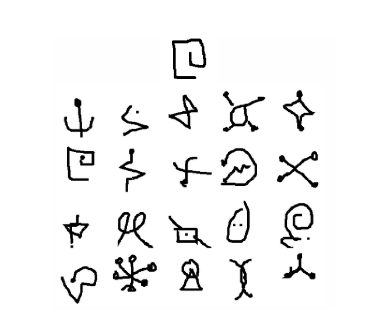
\includegraphics[width=0.4\textwidth]{background/omniglot_1_shot_20_way_task_example.png}
    \caption{A 1-shot, 20-way task from the Omniglot dataset \cite{omniglot}. The query sample is in top-center.}
    \label{figure:background:omniglot_sample}
\end{figure}

\subsection{Matching Networks}

While there is much previous research on few-shot approaches for deep learning, Matching Networks \cite{matchingnet} was the first to both train and test on n-shot, k-way tasks. The appeal of this is straightforward — training and evaluating on the same tasks lets us optimise for the target task in an end-to-end fashion. \\

Earlier approaches such as siamese networks use a pairwise verification loss to perform metric learning and then in a separate phase use the learnt metric space to perform nearest-neighbours classification. This is not optimal as the initial embedding function is trained to maximise performance on a different task! However, Matching Networks combine both embedding and classification to form an end-to-end differentiable nearest neighbours classifier. \\

Matching Networks first embed a high dimensional sample into a low dimensional space and then perform a generalised form of nearest-neighbours classification described by the equation below.

\begin{equation}
    \hat{y} = \sum_{i=1}^{k} a(\hat{x}, x_{i}) y_{i}
\end{equation}

The meaning of this is that the prediction of the model, $\hat{y}$, is the weighted sum of the labels, $y_i$, of the support set, where the weights are a pairwise similarity function, $a(\hat{x}, x_i)$, between the query example, $\hat{x}$, and a support set samples, $x_i$. The labels $y_i$ in this equation are one-hot encoded label vectors. \\

Notice that if we choose $a(\hat{x}, x_i)$ to be $\frac{1}{k}$ for the closest $k$ samples to the query sample and 0 otherwise we recover the k-nearest-neighbours algorithm. The key thing to note is that Matching Networks are end-to-end differentiable provided the attention function $a(\hat{x}, x_i)$ is differentiable. \\

The authors choose a straightforward softmax over cosine similarities in the embedding space as their attention function $a(x, x_i)$. The embedding function they use for their few-shot image classification problems is a CNN which is, of course, differentiable hence making the attention and Matching Networks fully differentiable! This means its straightforward to fit the whole model end-to-end with typical methods such as stochastic gradient descent.

\begin{equation}
a(\hat{x}, x_i) = \frac{e^{c(f(\hat{x}), g(x_i))}}{\sum_{j=1}^{k} e^{c(f(\hat{x}), g(x_i))}}
\end{equation}

In the above equation c represents the cosine similarity and the the functions f and g are the embedding functions for the query and support set samples respectively. Another interpretation of this equation is that the support set is a form of memory and upon seeing a new samples the network generates a prediction by retrieving the labels of samples with similar content from this memory. \\

Interestingly the possibility for the support set and query set embedding functions, f and g, to be different is left open in order to grant more flexibility to the model. In fact Vinyals et al. do exactly this and introduce the concept of full context embeddings or FCE for short. \\

They consider the myopic nature of the embedding functions a weakness in the sense that each element of the support set $x_i$ gets embedded by $g(x_i)$ in a fashion that is independent of the rest of the support set and the query sample. They propose that the embedding functions $f(\hat{x})$ and $g(x_i)$ should take on the more general form $f(\hat{x}, S)$ and $g(x_i, S)$ where S is the support set. The reasoning behind this is that if two of the support set items are very close, e.g. we are performing fine-grained classification between dog breeds, we should change the way the samples are embedded to increase the distinguishability of these samples. \\

In practice the authors use an LSTM to calculate the FCE of the support and then use another LSTM with attention to modify the embedding of the query sample. This results in an appreciable performance boost at the cost of introducing a bunch more computation and a slightly unappealing arbitrary ordering of the support set. \\

All in all this is a very novel paper that develops the idea of a fully differentiable neural neighbours algorithm.

\subsection{Prototypical Networks for Few Shot Learning}

\begin{figure}[H]
    \centering
    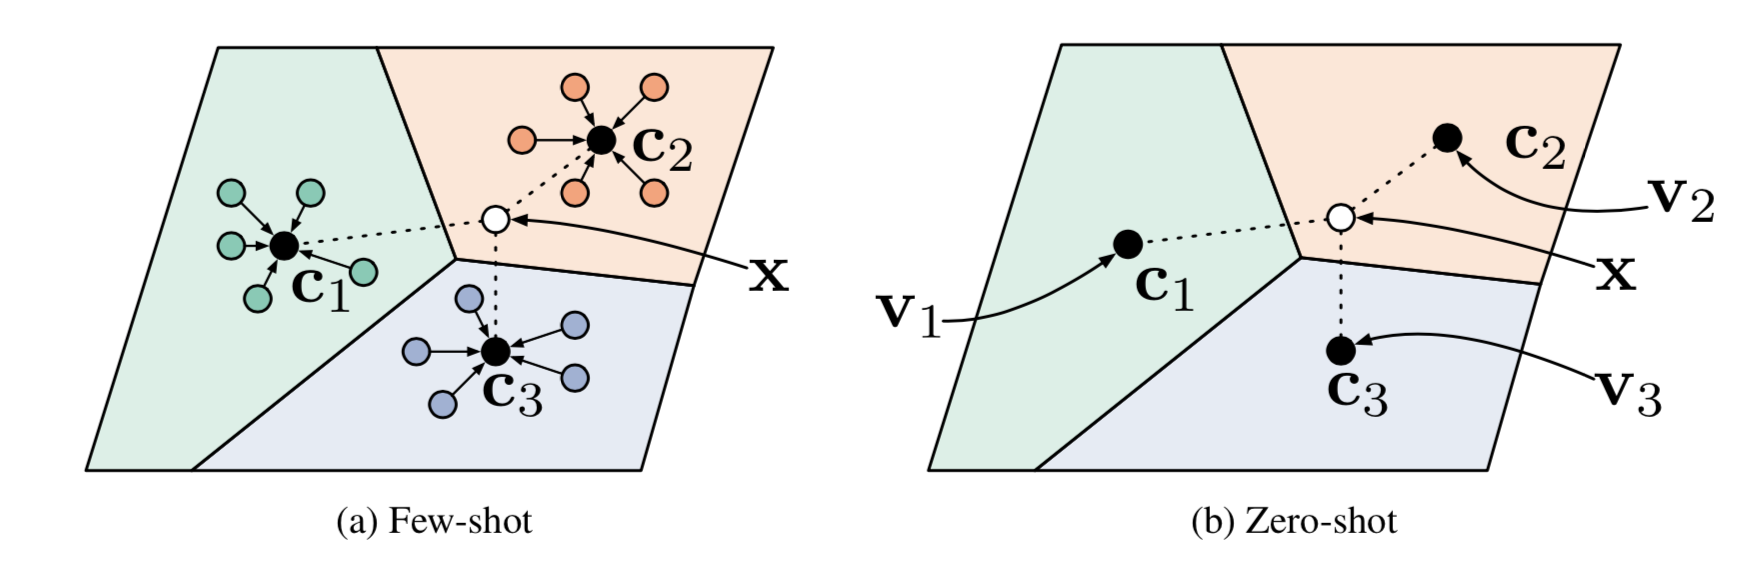
\includegraphics[width=0.8\textwidth]{background/prototypical-networks.png}
    \caption{Figure (1) of the paper. Prototypical networks in the few-shot and zero-shot scenarios. \textbf{Left}: Few-shot prototypes $c_k$ are computed as the mean of embedded support examples for each class. \textbf{Right}: Zero-shot
prototypes $c_k$ are produced by embedding class meta-data $v_k$. In either case, embedded query points are classified via a softmax over distances to class prototypes: \\ $p_{\phi}(y = k|x)$ $\alpha$ $e^{−d(f_{\phi}(x), c_k)}$.}
    \label{figure:background:prototypical}
\end{figure}

In Prototypical Networks \cite{protonet} Snell et al. apply a compelling inductive bias in the form of class prototypes to achieve impressive few-shot performance, exceeding Matching Networks without the complication of FCE. The key assumption is made is that there exists an embedding in which samples from each class cluster around a single prototypical representation which is simply the mean of the individual samples. This idea streamlines n-shot classification in the case of $n > 1$ as classification is simply performed by taking the label of the closest class prototype.

\begin{equation}
    c_k = \frac{1}{|S_k|} \sum_{(\mathbf{x}_i, y_i) \in S_k} f_{\phi}(\mathbf{x}_i)
\end{equation}
\captionof{figure}{Equation (1) from Prototypical Network calculating class prototypes. $S_k$ is the support set belonging to class $k$ and $f_{\phi}$ is the embedding function.}

Another contribution of this paper is a persuasive theoretical argument to use euclidean distance over cosine distance in metric learning that also justifies the use of class means as prototypical representations. The key is to recognise that squared euclidean distance (but not cosine distance) is a member of a particular class of distance functions known as Bregman divergences. \\

Consider the clustering problem of finding the centroid of a cluster of points such that the total distance between the centroid and all other points is minimised. It has been proven that if your distance function is a Bregman divergence (such as squared euclidean distance) then the centroid that satisfies this condition is simply the mean of the cluster, this is not the case for cosine distance however! This centroid is the point that minimises the loss of information when representing a set of points as just a single point. \\

                    This intuition is backed up by experiments as the authors find that both ProtoNets and their own implementation of Matching Networks are improved across the board by swaping from cosine to euclidean distance. \\

Prototypical Networks are also amenable to zero-shot learning, one can simply learn class prototypes directly from a high level description of a class such as labelled attributes or a natural language description. Once you’ve done this it’s possible to classify new images as a particular class without having seen an image of that class. In their experiments they perform zero-shot species classification of images of birds based only on attributes such as colour, shape and feather patterns.

\subsection{Dense Networks}

The development of neural networks is tending to make larger and wider networks. Many deep neural network models have been created in the latest years that follow this pattern. \\

Dense networks \cite{densenet} work by concatenating the feature-maps of a convolutional block to the feature-maps of all the previous convolutional blocks and using this value as input for the next convolutional block. This way each convolutional block is receiving all the collective knowledge of the previous layers maintaining the global state of the network which can be accessed from everywhere within the network. \\

Using this DenseNet architecture, the network can be thinner than ResNet but still giving better results. This is because of the feature reuse through the network which is a result of the input concatenation.
The original authors of DenseNet recommend using a small depth of the network with higher growth rate. This allows the network to obtain similar or better results in less time. This DenseNet is called Wide-Densenet and follow the strategy used by wide residual networks\cite{wide_resnet}.  \\

As our large model we selected Dense networks because it is shown that this model is one of the best achieving a 3.46\% error rate on Cifar10 over the 6.61\% error rate achieved with ResNet on the same dataset\cite{densenet_cifar}. This shows that DenseNet can handle small datasets with low error rate. This is thanks to its capacity of using features with multiple complexities in the classifier. \\

DenseNet also gets a lower error rate than ResNet in a larger dataset. With Cifar100 it achieved 17.18\% error rate over ResNet error rate of 20.50\%.

\subsection{Squeeze and Excitation blocks}

Convolutional networks construct informative features by fusion both spatial and chanel-wise information within local receptive fields at each layer. Squeeze and excitation blocks (SE block) \cite{senet} focus on the chanel-wise information used in the convolutional layers. \\

These SE blocks improve the quality of representations produced by the network by modelling the interdependency between channels and with this model doing feature recalibration. SE blocks can be included in every model that uses convolutional layers to improve its performance at low computational cost.

\begin{figure}[H]
    \centering
    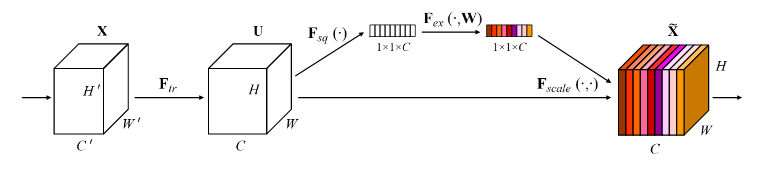
\includegraphics[width=0.8\textwidth]{background/se.png}
    \caption{}
    \label{figure:background:se}
\end{figure}

An SE block is a 2 step operation on a feature map V. First is the squeeze operation in which a global average pooling operation is performed reducing the dimensionality of V to a 2d vector with length equal to the amount of channels of V. Then the excitation operation is performed. This operation captures the inter-channel dependencies in a flexible (learning nonlinear interaction between channels) and non-mutually exclusive (we would like to ensure that multiple channels can be emphasised) way. The final output is obtained by making a channel wise multiplication between V and the scalar. This way we end with a feature map with weighted channels. \\

We included SE blocks in our dense network model after each dense block and transition block.

\begin{figure}[H]
    \centering
    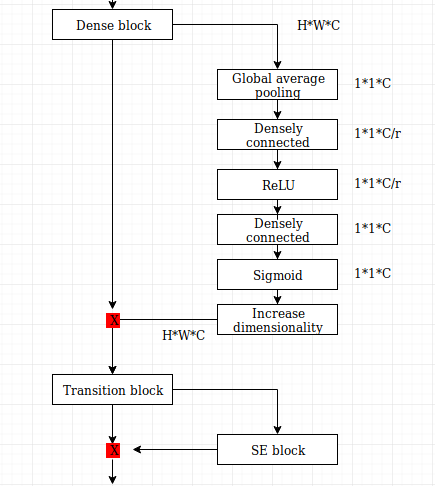
\includegraphics[width=0.8\textwidth]{background/sedense.png}
    \caption{}
    \label{figure:background:se}
\end{figure}

\subsection{Data Augmentation}

Image data augmentation is a set of techniques that aim at artificially augmenting the amount of data that can be obtained from the images in the dataset.  These techniques modify the images in the dataset creating new information that can be used as input for our model. \\

Using data augmentation we can work with fewer images having a lower variance lowering the chances of overfitting and having a better understanding of the most important features of each class in the dataset. Variance is defined by Abhijit Ghatak \cite{data_augmentation} as the tendency to learn random things irrespective of the real signal. Having a high variance implies that the model is learning from the noise of the data, in this case the model is overfitting. \\

For data augmentation we will apply flipping, rotation and rescaling on our images.